% Chapter Template

\chapter{Image processing} % Main chapter title

\label{Chapitre 4.1} % Change X to a consecutive number; for referencing this chapter elsewhere, use \ref{ChapterX}

\lhead{ \emph{Traitement des images}} % Change X to a consecutive number; this is for the header on each page - perhaps a shortened title

%----------------------------------------------------------------------------------------
%	SECTION 1
%----------------------------------------------------------------------------------------
Le but de cet exercice est de démontrer que l'on peut apprendre "n'importe quoi" à un réseau de neurone. Pour notre essai, nous allons apprendre à notre réseau de neurones la fonction : 


\section{Training data}


\begin{lstlisting}[frame=single,style=python]  % Start your code-block

x_train = [0:0.1:2*pi] ;
y_target = cos(x_train);
\end{lstlisting}


\begin{center} 
\hspace{15cm}
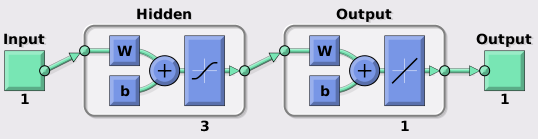
\includegraphics[width=15cm]{netview.png}
\end{center}
\vspace{0.5cm} 

On voit que l'on à qu'une entrée et une sortie, ce qui est logique, car on veut entrer une valeur de "x" et obtenir le cosinus de "x". Le type d'entrainement utilisé est "Levenberg-Marquardt".\\

Voici le diagramme MSE généré par notre outils : 

\begin{center} 
\hspace{15cm}
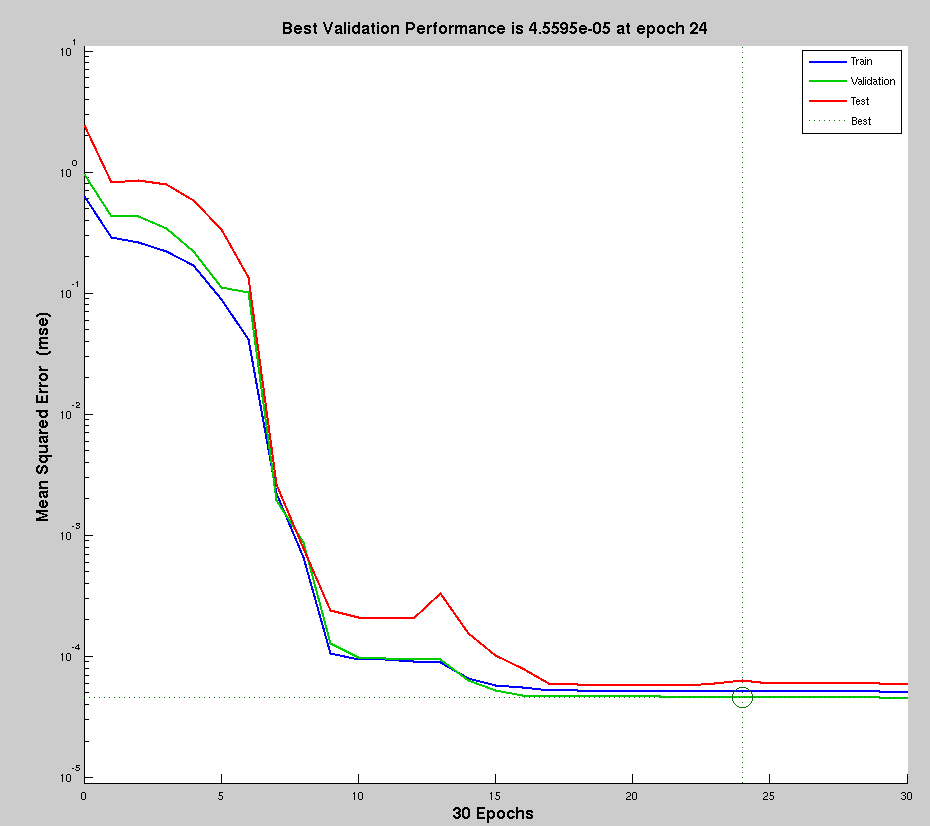
\includegraphics[width=10cm]{mse_cos.png}
\end{center}
\vspace{1cm}
On peut bien voir le travail d'entrainement et le calcul des poids pour minimiser l'erreur. Vérifions maintenant notre système.
\pagebreak


\section{Vérification}

Afin de vérifier si notre système fonctionne, on génère maintenant une nouvelle série des valeur de "x" qui n'appartiennent pas à l'ensemble d'entrainement. Voilà le code :

\begin{lstlisting}[frame=single,style=C]  % Start your code-block

x_validation = [0:0.03:2*pi];

y = net(x_validation);
y10 = net10(x_validation);
\end{lstlisting}

Voilà le résultat (en haut la sortie y, et en bas l'erreur par rapport au vrai cos(x)) : 
\begin{center} 
\hspace{15cm}
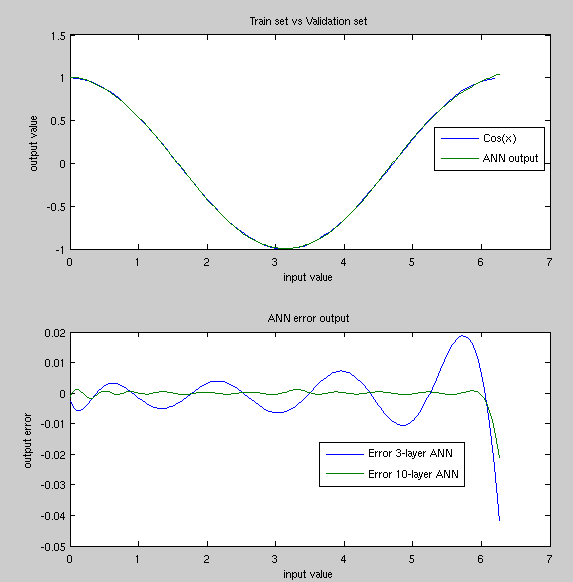
\includegraphics[width=15cm]{cos_res.png}
\end{center}
\vspace{1cm}


On voit que l'on à bien pu entrainer notre système avec $x \in [0;2\pi]$ (au-delà le système est faux, l'erreur grandit). On voit que le système à 10 layers est nettement plus performant que le système à 3 layers. Toutefois, le système devient instable pour des valeurs de $x$ approchant $2\pi$.   